\documentclass[a4paper,10pt]{article}

        \addtolength{\oddsidemargin}{-0.5in}
        \addtolength{\evensidemargin}{-0.5in}
        \addtolength{\textwidth}{1in}

\setlength{\parindent}{0pt}% remove indents before paragraphs

\usepackage[english]{babel}
\usepackage[utf8x]{inputenc}

% Some useful packages.
\usepackage{amsmath,amssymb}
\usepackage{mathtools}
\usepackage{enumerate}
\usepackage{float}
\usepackage[justification=centering]{caption}
\usepackage{mathtools}
% Commands for basic statistics.
\DeclareMathOperator{\E}{\mathbb{E}}
\DeclareMathOperator{\Var}{Var}
\DeclareMathOperator{\Cov}{Cov}

\begin{document}

\title{Information visualization \\ Assignment 1}
\author{Ari Viitala 432568}
\maketitle

\section*{Exercise 1}
\subsection*{a)}
In the original visualization by NASA there are many things that contradict Tufte's principles of graphical excellence. First of all there is much ink spent on little information. For example all the boosters that have no problems during launch use up 2 images of boosters only to tell the temperature during launch. Also the running index numbers of different launches and the alternating A and B labels for different boosters are pretty useless since any sensible person would realize which is booster A and which is booster B if it would be told just once instead of 24 times. All these things mean that the data-ink ratio in the visualization is pretty bad. 
\\\\
Also in my opinion the rocket boosters count as chart junk since there is surely a better way to visualize where on the rocket the leak happened without drawing the entire booster. Furthermore the extra boosters take up extra space making the whole image take up more space than it should which is also against Tufte's principles. One more thing that fights against Tufte's principles is the amount of gas leaked from the O-ring is shown with different types of dots and lines. I understand that this makes it interpretable in a black and white print but it also is in my opinion a bit ambiguous and fall's into the category of showing variation in design and not in data. And if not that then at least it is ambiguous.
\\\\
Also the graph does a pretty bad job at communicating the relationship of the O-ring temperature with the gas leaks since there is really no cause and effect visible. The viewer has to manually compare each temperature and the outcome of the launch in order to see the relationship instead of just seeing it right away. 

\subsection*{b)}

In figure \ref{launch} is presented a better visualization for investigating the relationship between the O-ring temperature and the risk for an accident. In this graph we have scrapped the useless rocket figures since the goal is not to investigate where an accident happened. Every accident is not favorable so we are interested what is the worst thing that happened during the launch and not the specific location. Also the 

\begin{figure}
\centering
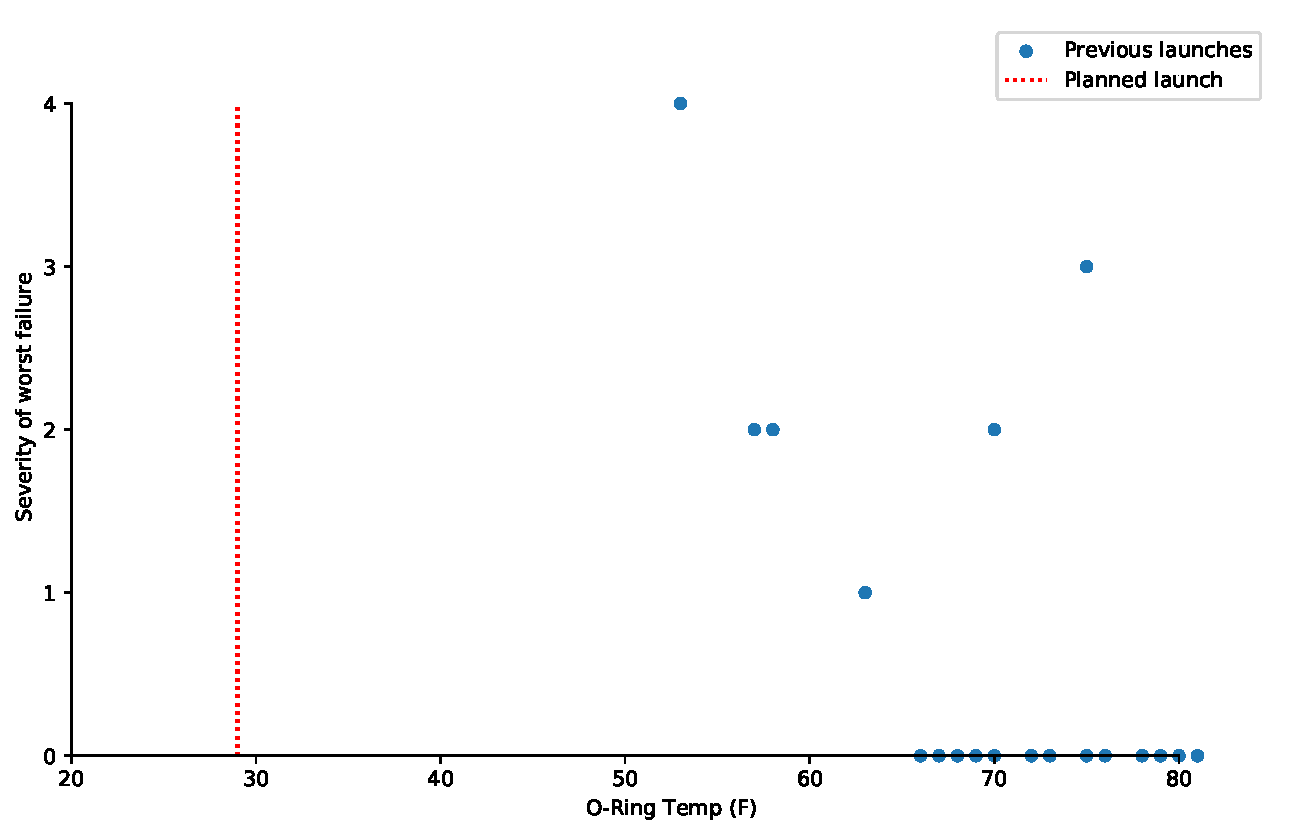
\includegraphics[width = \linewidth]{launch}
\caption{The most severe accident of the launch as the function of O-ring temperature as well as the planned launch at 29 degrees Farenheit}
\label{launch}
\end{figure}

\section*{Exercise 2}

I found the visualization that can be seen in figure \ref{Hesari} from Helsingin Sanomat web page and I think it is pretty bad. First of all the whole graph represents only 9 pieces of information but the whole image is so large that it didn't even fit on my computer screen. This means that there is a lot of ink but not too much data. Also the sizes of the exports is represented with balls which isn't really informative and also I'm pretty sure that the sizes of the balls are wrong since the red should be about twice as big as the yellow but I think it is more than twice larger or at least it looks like it. Furthermore, down at the bottom of the image is the size of export as a percentage of the whole export. Of course the point of the graph is to tell how the possible steel tariffs to the US would affect certain regions but in my opinion it is even misleading to tell only the percentage values since China is no big. I think they should have also included the absolute values of the export to the Nafta region.
\\\\
The image would be much better for example as a simple bar plot where the height of the bar is the absolute value of steel export and one segment could be colored with other color to represent the amount of export going to the Nafta region. The you could add the percentage value also if you deemed that necessary. This type of visualization would make it much faster to interpret the image and in my opinion it would be more truthful way of conveying the current situation while retaining the amount of data. 

\begin{figure}[h!]
\centering
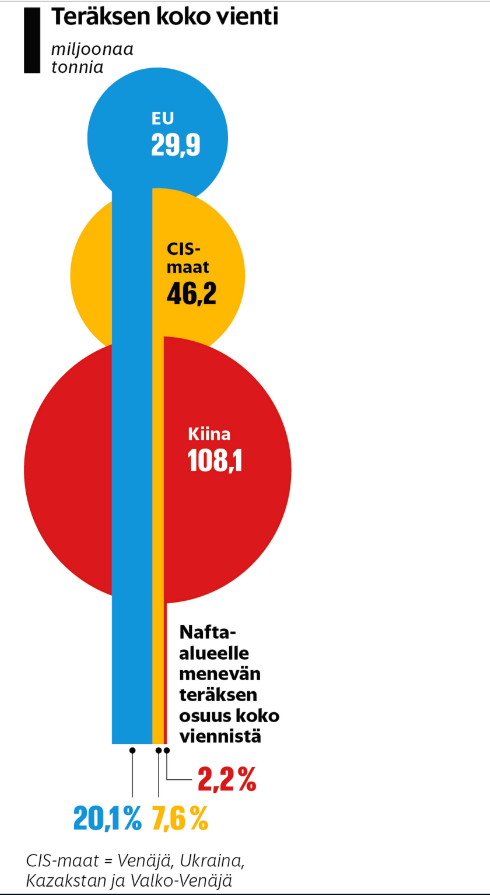
\includegraphics[width = 10cm]{hesari}
\caption{An illustration of steel exports for EU, CIS countries and China to Nafta region}
\label{Hesari}
\end{figure}

\section*{Exercise 3}

\subsection*{a)}
In figure \ref{Bitcoinbetter} there are plotted the 20 day rolling averages of S\&P 500 index and the Price of Bitcoin which are indexed to 100 index points at 13.3.2015. We can clearly see that Bitcoin has clearly outperformed S\&P 500 since the year 2016. Coming up to year 2018 the price of Bitcoin has risen nearly 5000\% whereas S\&P has seen practically no growth in that time frame. 
\begin{figure}
\centering
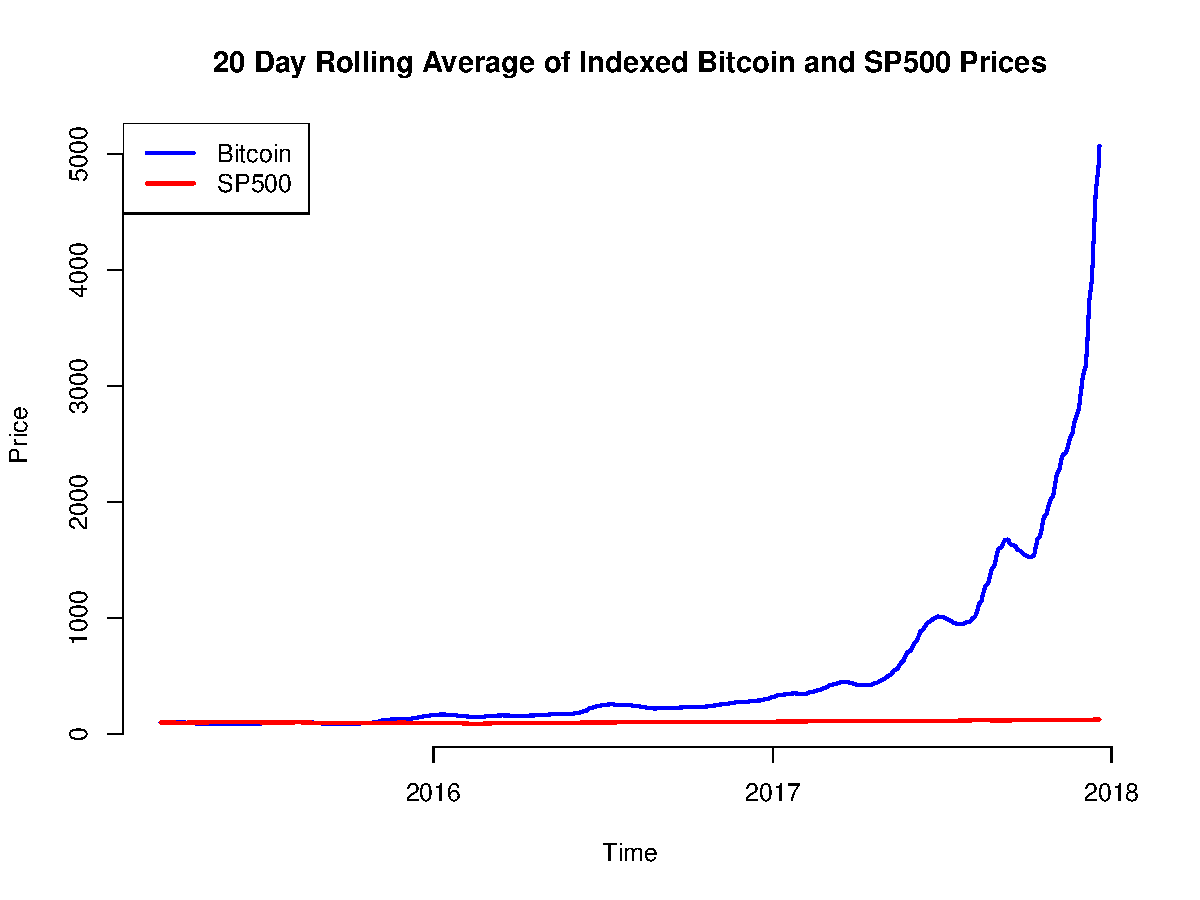
\includegraphics[width = 11cm]{bitcoin_better}
\caption{Comparison of 20 day rolling average of Bitcoin and SP500 prices indexed to 100 points at 13.3.2015}
\label{Bitcoinbetter}
\end{figure}

\subsection*{b)}

In figure \ref{spbetter} we can clearly see that the S\&P 500 index is much better in bringing constant profit to investors. Bitcoin has just recently spiked and is going down as fast as it went up but S\&P 500 index keeps going up like it has for years. 

\begin{figure}
\centering
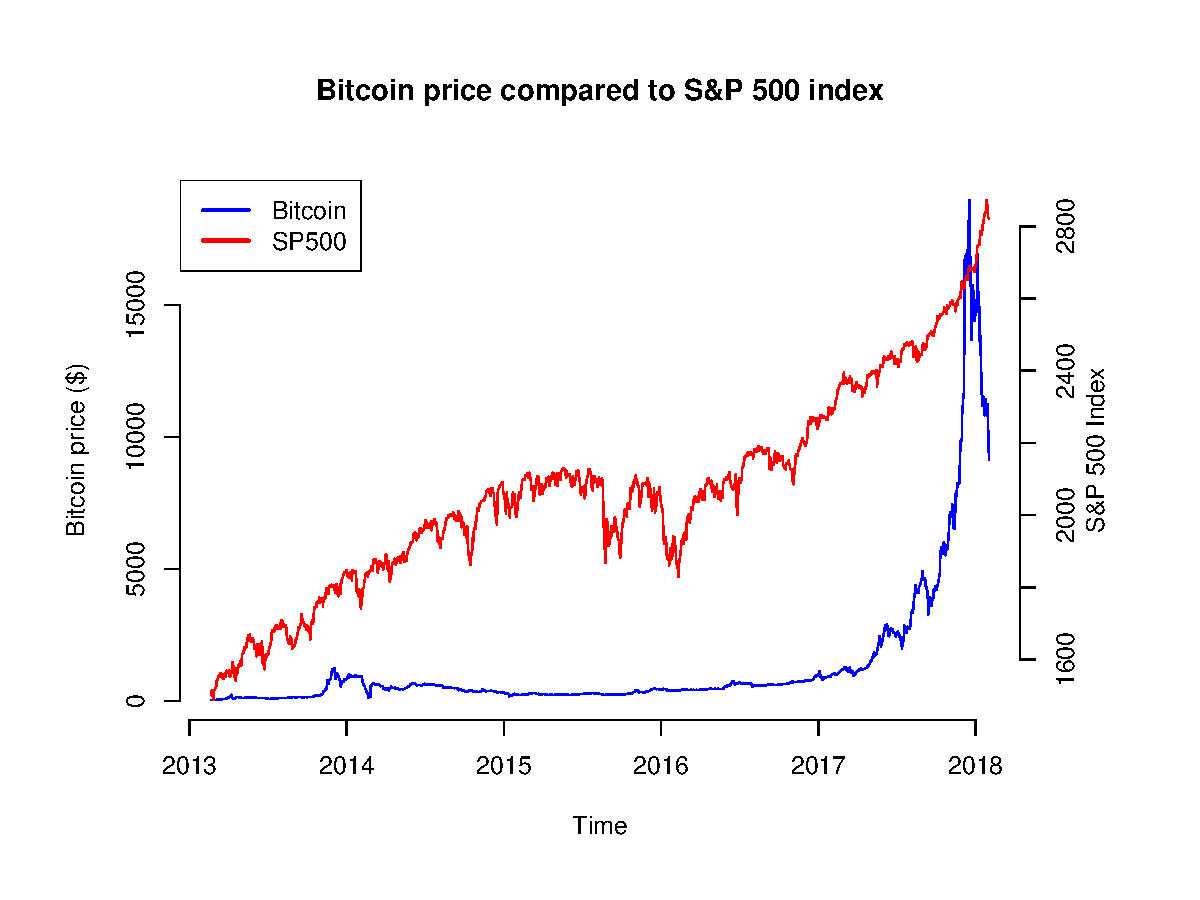
\includegraphics[width = 13cm]{sp_better}
\caption{Bitcoin price and S\&P 500 index since the year 2013}
\label{spbetter}
\end{figure}

\subsection*{c)}
In the figure \ref{Bitcoinbetter} the lie factor could as well be approaching infinity since in the graphic it seems like SP500 is not increasing at all where as Bitcoin is soaring so the difference in growth rates goes to infinity as well as the lie factor. Well, in any case the lie factor is really large since Bitcoin price grows so much faster than the index.
\\\\
In the figure \ref{spbetter} the lie factor is much smaller but still pretty big. In reality reality Bitcoin has risen 30000\% since the year 2013 where as the index has only doubled so the rise in S\%P 500 is 15000\% smaller in the data whereas in the graph they are equal. This means that the lie factor is 
\begin{equation}
\textit{Lie factor } = \frac{\textit{Effect in graph}}{\textit{Actual effect}} = \frac{1}{\frac{1}{150}} = 150.
\end{equation}

\subsection*{d)}

\begin{figure}
\centering
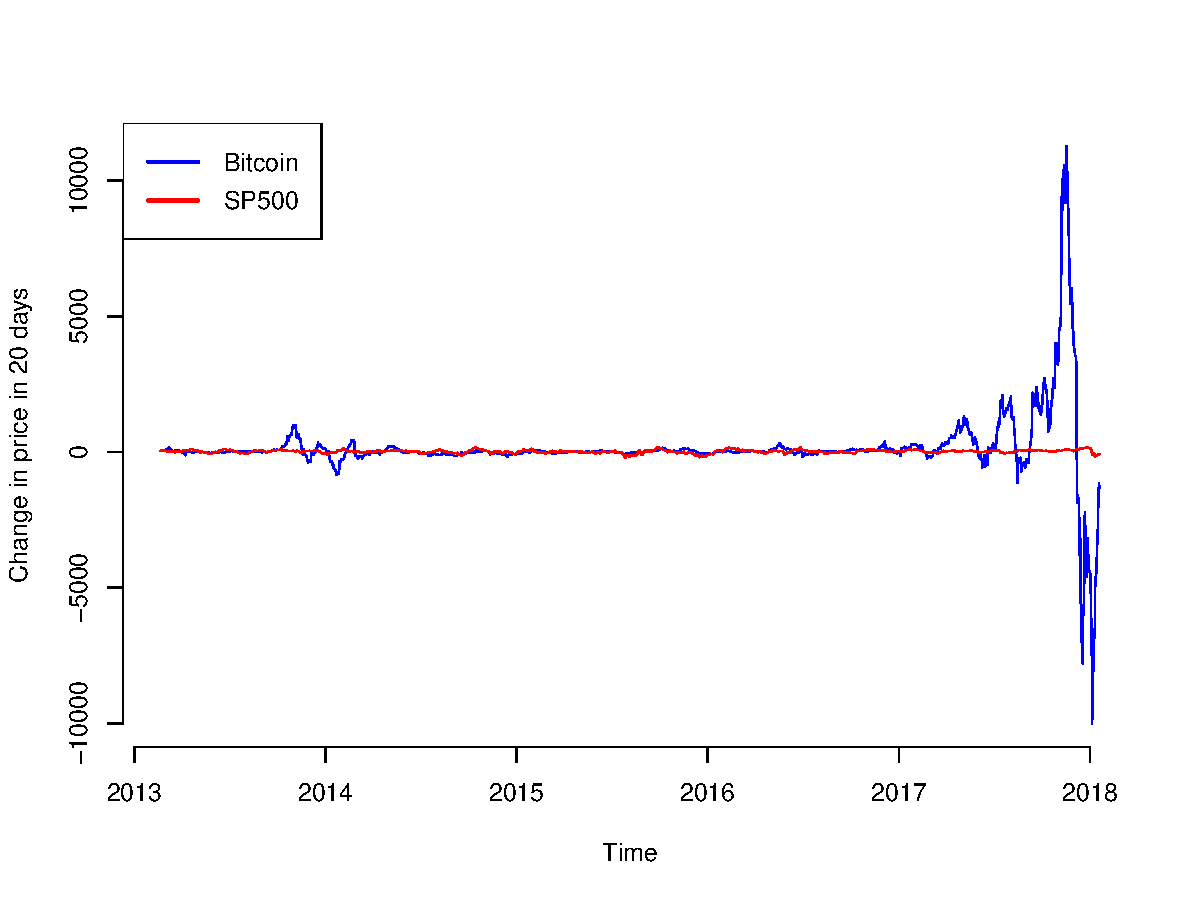
\includegraphics[width = \linewidth]{Honesplot}
\caption{The price change in twenty days for both}
\end{figure}

\newpage
\section{Exercise 4}

In figure \ref{Lipds} there are plotted four different lipids from olives from different regions. We see that region 1 is easy to distinguish from eiconsenonic lipid because the other regions seem to have none of it. Region three is easy to distinguish from plots between oleic and linolenic or linoleic and linolenic since it has a really discrete distribution. Region 2 is not really clearly distinguished from the images but if we recognize regions one and three then region 2 is ten one that is left out. 
\begin{figure}[h!]
\centering
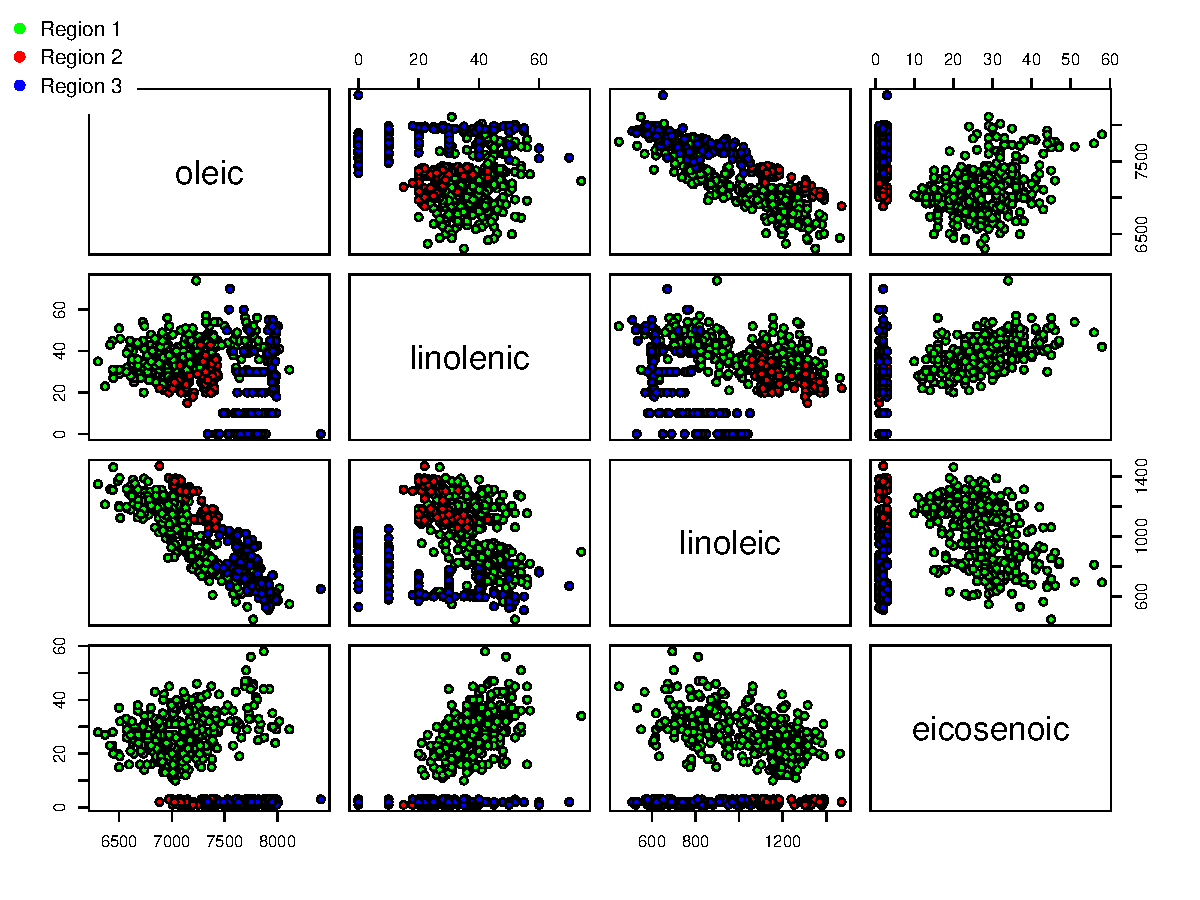
\includegraphics[width = \linewidth]{trellis}
\caption{Four different lipids from olives from different regions}
\label{Lipds}
\end{figure}
\end{document}